\documentclass{beamer}
\usetheme[
  block=fill, 
  background=dark,
  titleformat=smallcaps,
  progressbar=frametitle,
  numbering=none,
]{metropolis}

%----------------------------------------------------------------------------
% From dyck-paper
%----------------------------------------------------------------------------
\usepackage{mwe,tikz}\usepackage[percent]{overpic}
\usepackage{caption}
\usepackage{epigraph}
% Math
\usepackage{amsmath}
\usepackage{amssymb}
\usepackage{stmaryrd}
% Code listing
\usepackage{minted}
%\usemintedstyle{friendly}
\usemintedstyle{tango}
\usepackage{algorithm}
\usepackage[noend]{algpseudocode}
% Colors
\usepackage{xcolor}
\colorlet{CodeBg}{gray!90}
\usepackage{color, colortbl}
\definecolor{Gray}{rgb}{0.9,0.9,0.9}
\definecolor{bblue}{HTML}{1D577A}
\definecolor{rred}{HTML}{C03425}
\definecolor{ggreen}{HTML}{8BB523}
\definecolor{ppurple}{HTML}{6B1B7F}
\definecolor{pblack}{HTML}{000000}
\definecolor{pyellow}{HTML}{C0B225}
% Graphs
\usepackage{tikz}
\usetikzlibrary{calc}
\usetikzlibrary{trees}
\usetikzlibrary{positioning}
\usepackage{pgfplots}
% Graphics
\usepackage{graphics}
\graphicspath{{figures/}} % Location of the graphics files

\newcommand\todo[1]{\textcolor{red}{#1}}
\newcommand{\w}[1]{\textit{"#1"}}
\newcommand{\sm}[1]{\text{\small{#1}}}
\newcommand\s{\textsc}

\newcommand{\Order}[5]{
	\[
	\mathcal{#1}_{#5}\llbracket #2 \leftarrow #3 \mid \{ #4 \} \rrbracket.
	\]
}
\newcommand{\Orderr}[5]{
	\mathcal{#1}_{#5}\llbracket #2 \leftarrow #3 \mid \{ #4 \} \rrbracket.
}
\newcommand{\Ord}[4]{\Order{O}{#1}{#2}{#3}{#4}}
\newcommand{\Or}[4]{\Orderr{O}{#1}{#2}{#3}{#4}}
\newcommand{\Con}[4]{\Order{C}{#1}{#2}{#3}{#4}}

% Box macro
\newcommand{\ex}[2]{
  \vfill
  \begin{alertblock}{#1}
    #2
  \end{alertblock}
}
\newcommand\tsc[1]{\alert{\textsc{#1}}}

%\setbeamercolor{alerted text}{%
%  fg=ggreen
%}
%----------------------------------------------------------------------------

% Beamer
\title{$D^3$ as a 2-MCFL}
\subtitle{}
\author{Orestis Melkonian, Konstantinos Kogkalidis}
\date{January 25, 2018}
\institute{Universiteit Utrecht}

\begin{document}
	\maketitle
	
	\begin{frame}{}
	\begin{center}
	\vspace{1cm}
	\colorbox{white}{
    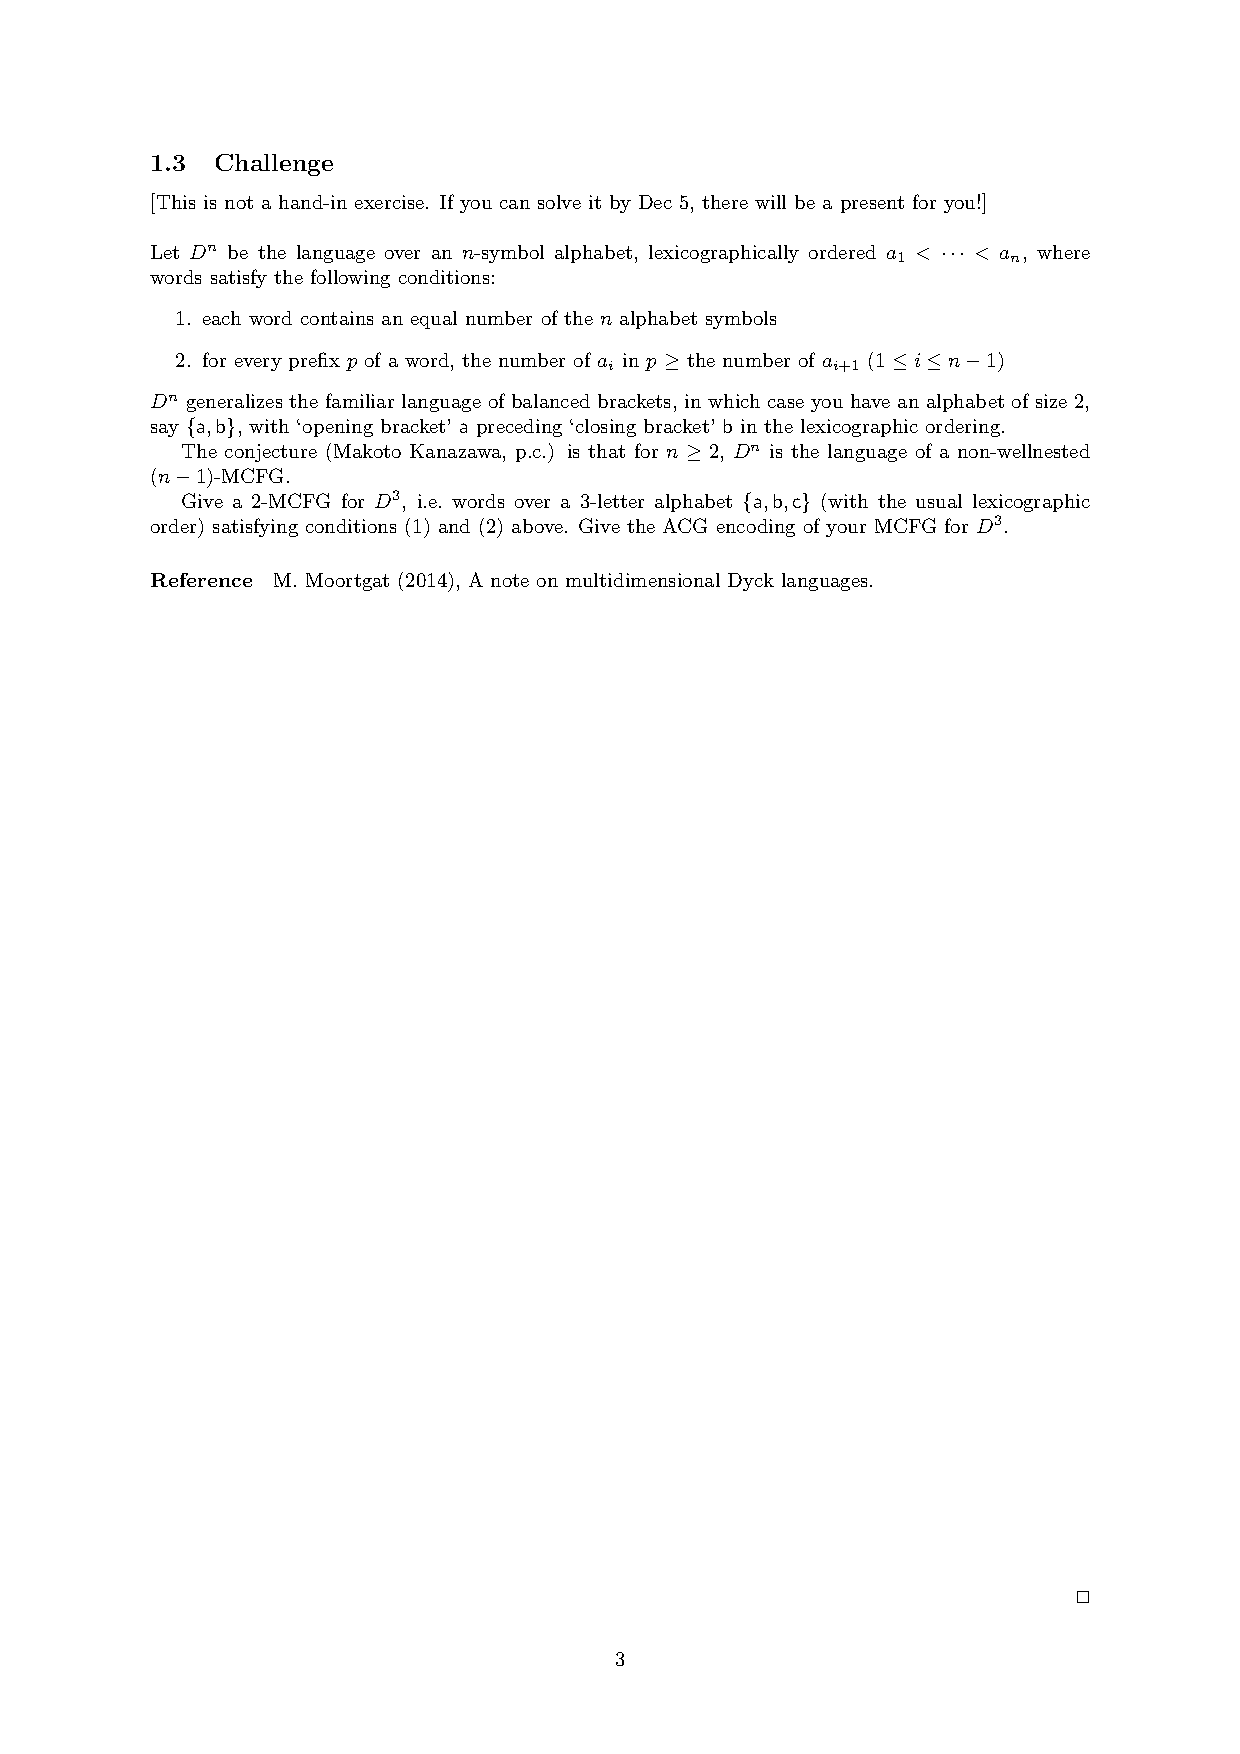
\includegraphics[clip, trim=1cm 18cm 1cm 1cm, scale=.55]{quiz.pdf}}
	\end{center}
	\end{frame}

%	\begin{frame}{}
%		\epigraph
%			{When you depart for Ithaca,\\wish for the road to be long,\\full of adventure, full of knowledge.}
%			{\textit{C. P. Cavafy\\ Ithaca}}
%	\end{frame}

	\begin{frame}{Some examples}
		\hspace{1cm}
		\begin{minipage}{.4\textwidth}
		\textsc{Dyck words}
		\begin{itemize}
			\item \textcolor{ggreen}{abc}
			\item \textcolor{ggreen}{aabbcc}
			\item \textcolor{ggreen}{abcabcabacbc}
		\end{itemize}	
		\end{minipage}
		\pause
		\begin{minipage}{.4\textwidth}
		\textsc{Non-dyck words}
		\begin{itemize}
			\item \textcolor{rred}{aabb}
			\pause
			\item \textcolor{rred}{aabbbcc}
			\pause
			\item \textcolor{rred}{abcacb}
		\end{itemize}	
		\end{minipage}
		\vspace{1cm}
		\pause
		\begin{figure}[h!]
		\centering
		
\begin{tikzpicture}[every node/.style={anchor=base},xscale=.25,yscale=.4]
			\node (n0) at (0,0) {$a$};
			\node (n1) at (1,0) {$b$};
			\node (n2) at (2,0) {$a$};
			\node (n3) at (3,0) {$b$};
			\node (n4) at (4,0) {$a$};
			\node (n5) at (5,0) {$c$};
			\node (n6) at (6,0) {$b$};
			\node (n7) at (7,0) {$c$};
			\node (n8) at (8,0) {$a$};
			\node (n9) at (9,0) {$b$};
			\node (n10) at (10,0) {$c$};
			\node (n11) at (11,0) {$c$};
			\pause
			\draw (n0) edge [thick, rred, bend left=90] (n1);
			\draw (n1) edge [thick, rred, bend right=90] (n5);
			\pause
			\draw (n2) edge [thick, ggreen, bend left=90] (n3);
			\draw (n3) edge [thick, ggreen, bend right=90] (n7);
			\pause
			\draw (n4) edge [thick, bblue, bend left=90] (n6);
			\draw (n6) edge [thick, bblue, bend right=90] (n10);
			\pause
			\draw (n8) edge [thick, pyellow, bend left=90] (n9);
			\draw (n9) edge [thick, pyellow, bend right=90] (n11);
		\end{tikzpicture}
		\caption*{First-match policy}
		\end{figure}
	\end{frame}
	
	\begin{frame}{G$_0$: Grammar of triple insertions}
		\begin{figure}[h!]
		\begin{align}
		\setcounter{equation}{0}
		\s{S}(xy) \leftarrow \s{W}(x,y)&. \\
		\s{W}(\epsilon, xy\textbf{abc}) \leftarrow \s{W}(x,y)&. \\
		\s{W}(\epsilon, x\textbf{a}y\textbf{bc}) \leftarrow \s{W}(x,y)&. \\
		...... \nonumber \\
		\setcounter{equation}{59}
		\s{W}(\textbf{ab}x\textbf{c}y, \epsilon) \leftarrow \s{W}(x,y)&. \\
		\s{W}(\textbf{abc}xy, \epsilon) \leftarrow \s{W}(x,y)&. \\
		\s{W}(\epsilon, \textbf{abc})&. \\
		\s{W}(\textbf{a}, \textbf{bc})&. \\
		\s{W}(\textbf{ab}, \textbf{c})&. \\
		\s{W}(\textbf{abc}, \epsilon)&.
		\end{align}
		\end{figure}
	\end{frame}
	
	\begin{frame}{G$_0$: Grammar of triple insertions}
		\begin{figure}[h!]
		\centering
		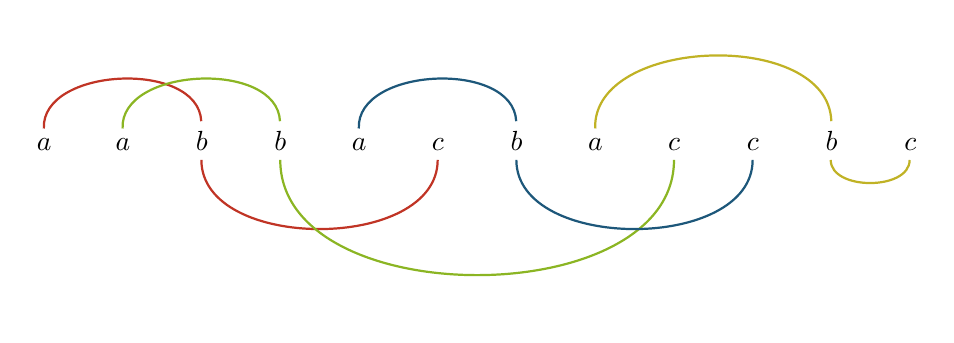
\begin{tikzpicture}[every node/.style={anchor=base}]
			\node (n0) at (0,0) {$a$};
			\node (n1) at (1,0) {$a$};
			\node (n2) at (2,0) {$b$};
			\node (n3) at (3,0) {$b$};
			\node (n4) at (4,0) {$a$};
			\node (n5) at (5,0) {$c$};
			\node (n6) at (6,0) {$b$};
			\node (n7) at (7,0) {$a$};
			\node (n8) at (8,0) {$c$};
			\node (n9) at (9,0) {$c$};
			\node (n10) at (10,0) {$b$};
			\node (n11) at (11,0) {$c$};
			\pause
			\draw (n0) edge [thick, rred, bend left=90] (n2);
			\draw (n2) edge [thick, rred, bend right=90] (n5);
			\pause
			\draw (n1) edge [thick, ggreen, bend left=90] (n3);
			\draw (n3) edge [thick, ggreen, bend right=90] (n8);
			\pause
			\draw (n4) edge [thick, bblue, bend left=90] (n6);
			\draw (n6) edge [thick, bblue, bend right=90] (n9);
			\pause
			\draw (n7) edge [thick, pyellow, bend left=90] (n10);
			\draw (n10) edge [thick, pyellow, bend right=90] (n11);
		\end{tikzpicture}
		\caption*{Straddling counter-example}
		\end{figure}
	\end{frame}
  	
  	\begin{frame}{Meta-grammars: Introduction}
	  	\vspace{.7cm}
	  	\center \tsc{Notation}
  		\[
  			\Or{conclusion}{premises}{partial\ orderings\ of\ inserted\ elements}{m}
  		\]
  		\vspace{.1cm}
  		\pause
  		\begin{center}\tsc{Meta-grammar G$_1$}\end{center}
  		  \[ \left . \ \begin{array}{ll}
					\Or{W}{\epsilon}{a < b < c}{2} \\
                \Or{W}{W_{xy}}{x < y,\ a < b < c}{2}
           \end{array}
           \right\} \textsc{triple insertion}
		  \]
  		\pause
  		\hspace{-4cm}\textcolor{ggreen}{+}
  		\[ \left . \ \hspace{-3cm}\begin{array}{ll}
					\Or{W}{W_{xy}, W_{zw}}{x < y,\ z < w}{2}
         \end{array}
         \right . \
		\]
  		\vspace{.7cm}
  	\end{frame}
  	
  	\begin{frame}{G$_2$: Adding states}
   	\small
   	\begin{flalign*}
 		&\left . \ \begin{array}{lr}
					\Or{A^+}{\epsilon}{a}{2} \\
					\Or{B^+}{\epsilon}{b}{2} \\
					\Or{C^+}{\epsilon}{c}{2}
           \end{array}
           \right\} \tsc{base cases} \\
  		&\noindent\rule{11cm}{0.4pt}\\
 		&\left . \ \begin{array}{lr}
					\Or{C^-}{A^+, B^+}{x < y < z < w}{2} \\
					\Or{B^-}{A^+, C^+}{x < y < z < w}{2} \\
					\Or{A^-}{B^+, C^+}{x < y < z < w}{2} \\
					\Or{A^+}{C^-, B^-}{x < y < z < w}{2} \\
					\Or{B^+}{C^-, A^-}{x < y < z < w}{2} \\
					\Or{C^+}{B^-, A^-}{x < y < z < w}{2} \\
					\forall \ \s{K} \in \mathcal{S} \setminus \s{W}:\ \Or{\s{K}}{\s{K}_{xy}, \s{W}_{zw}}{x < y,\ z < w}{2}
           \end{array}
           \right\} \tsc{combinations} \\
		&\noindent\rule{11cm}{0.4pt}\\
  		&\left . \ \begin{array}{lr}
					\Or{W}{A^+, A^-}{x < y < z < w}{2} \\
					\Or{W}{C^-, C^+}{x < y < z < w}{2}
           \end{array}
           \right\} \tsc{closures}
	\end{flalign*}
  	\end{frame}
  	
  	\begin{frame}{G$_3$: G$_2$ + Universal triple insertion}
  	\begin{align*}
  		&\text{G}_3 = \text{G}_2\ \textcolor{ggreen}{+}\ \forall \ \s{K} \in \mathcal{S} \setminus \s{W}:\\ 
&\hspace{3cm}\Or{\s{K}}{\s{K}_{xy}}{x < y,\ a < b < c}{2}
  	\end{align*}
  	\end{frame}

{\usebackgroundtemplate{%
  
\includegraphics[width=\paperwidth,height=\paperheight]{demo.png}}
	\begin{frame}{Demo}
	   \centering   
	   \begin{overpic}[scale=0.3]{demo.png}
	     \put(20,10){
\includegraphics[scale=0.2]{demo.png}} 
	     \put(35,20){
\includegraphics[scale=0.1]{demo.png}}
	   \end{overpic}
  	\end{frame}
}
  	
  	\begin{frame}{Refining states I}
  		\center \tsc{Example}
  		\begin{figure}[h!]
		\centering
		\begin{tikzpicture}[every node/.style={anchor=base}]
			\node (c) at (0,0) {$A^{+}(x, y)$};
			\node (l) at (-2,-1) {$A^{+}_{left}(\dots a\dots ,\ \dots)$};
			\node (r) at (2,-1) {$A^{+}_{right}(\dots,\ \dots a\dots)$};
			\draw (c) edge [->, mLightBrown, thick] (l);
			\draw (c) edge [->, mLightBrown, thick] (r);
		\end{tikzpicture}
		\end{figure}
		\center \tsc{Why? \pause \\New orders in interactions}
		\[ C^-(xz,\ wy) \leftarrow A^{+}_{left}(x,\ y),\ B^{+}_{left}(z,\ w).
		\]
  	\end{frame}
  	
  	\begin{frame}{Refining states II}
  		\centering
		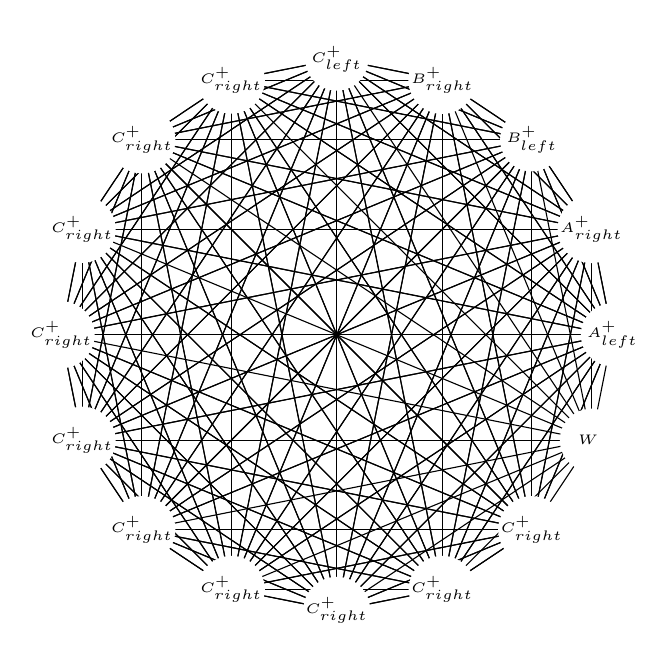
\begin{tikzpicture}[scale=.7]
		  \foreach \x /\alph/\name in {
		  		0/n1/$A^{+}_{left}$,
		  		22.5/n2/$A^{+}_{right}$,
		  		45/n3/$B^{+}_{left}$,
		  		67.5/n4/$B^{+}_{right}$,
		  		90/n5/$C^{+}_{left}$,
		  		112.5/n6/$C^{+}_{right}$,
		  		135/n7/$C^{+}_{right}$,
		  		157.5/n8/$C^{+}_{right}$,
		  		180/n9/$C^{+}_{right}$,
		  		202.5/n10/$C^{+}_{right}$,
		  		225/n11/$C^{+}_{right}$,
		  		247.5/n12/$C^{+}_{right}$,
		  		270/n13/$C^{+}_{right}$,
		  		292.5/n14/$C^{+}_{right}$,
		  		315/n15/$C^{+}_{right}$,
		  		337.5/n16/$W$
		  }{
		  	\node[] (\alph) at (\x:5cm) {};
		  }		
		  \foreach \alpha in {n1,n2,n3,n4,n5,n6,n7,n8,n9,n10,n11,n12,n13,n14,n15,n16}%
		  {%
		  \foreach \alphb in {n1,n2,n3,n4,n5,n6,n7,n8,n9,n10,n11,n12,n13,n14,n15}%
		  {%
		   \draw (\alpha) edge (\alphb);%
		  }}
		  \foreach \x /\alph/\name in {
		  		0/n1/$A^{+}_{left}$,
		  		22.5/n2/$A^{+}_{right}$,
		  		45/n3/$B^{+}_{left}$,
		  		67.5/n4/$B^{+}_{right}$,
		  		90/n5/$C^{+}_{left}$,
		  		112.5/n6/$C^{+}_{right}$,
		  		135/n7/$C^{+}_{right}$,
		  		157.5/n8/$C^{+}_{right}$,
		  		180/n9/$C^{+}_{right}$,
		  		202.5/n10/$C^{+}_{right}$,
		  		225/n11/$C^{+}_{right}$,
		  		247.5/n12/$C^{+}_{right}$,
		  		270/n13/$C^{+}_{right}$,
		  		292.5/n14/$C^{+}_{right}$,
		  		315/n15/$C^{+}_{right}$,
		  		337.5/n16/$W$
		  }{
		  	\node[circle,inner sep=0pt,minimum size=8mm,fill=white] (\alph) at (\x:5cm) {\tiny \textcolor{black}{\name}};
		  }	
		 \end{tikzpicture}
  	\end{frame}
  	\begin{frame}{Automatic Rule Inference System}
  	\end{frame}
  	
  	
  	\begin{frame}{Overview}
    \begin{itemize}
      \item Background
      \item $G0$: Triple insertion
      \item Meta-grammar notation
      \item $G_0'$: Triple insertion (in $O_2$ notation)
      \item $G_1$: G0' + interleavings
      \item $G_2$: incomplete words
      \item $G_3$: G2 + 3-ins
      \item \alert{DEMO}: \textbf{dyck}
      \item Refined states
      \item Constraints (notation)
      \item ARIS
      \item Results
      \item Road to completeness
      \item Correspondences
      \item \alert{DEMO}: \textbf{dyckviz}
    \end{itemize}
	\end{frame}
\end{document}